%In this section, we will explore the causes of the high risk of losses in accessibility for Pacifica, CA.
%Like Danville, Pacifica is at high risk of losses in accessibility, but for different reasons.
%While trip length and bridge vulnerability play a big role in the accessibility risk for Danville, physical conditions contribute significantly to the risk of Pacifica, CA (Figure~\ref{fig:equity_study_area}). \textcolor{red}{TODO: write section}
%In contrast to downtown San Francisco, Pacifica, CA  (Figure~\ref{fig:equity_study_area}) has a high risk of losses in accessibility. We will now explore why. 

%Based on seismic hazard (e.g., Figures~\ref{fig:haz475} and \ref{fig:haz2475}), we might not suspect that Pacifica, CA would be at an elevated risk of accessibility losses across most market segments. In addition, the percentage of pre-earthquake car-based trips is around average for the case study area (88\% versus an average of 85\%). 
%In contrast to most other regions, however, Pacifica is wedged between the Pacific Ocean to the West and the coastal mountains to the East. Indeed, the main access road is California Highway 1, which has various vulnerable bridges included in the case study dataset. There are no viable alternative routes on local roads. Since almost all trips are by car from Pacifica and the average trip length is much longer than the region-wide average (108\% longer), the road issue is particularly serious.

We might not suspect that Pacifica, CA would be at an extremely elevated risk of accessibility losses across most market segments, as compared to other communities, because it is not unusually close to a major earthquake fault. In addition, the percentage of pre-earthquake car-based trips is around average for the case study area (88\% versus an average of 85\%). 
In contrast to most other regions, however, Pacifica is wedged between the Pacific Ocean to the West and the coastal mountains to the East. Indeed, the main access road is California Highway 1, which has various vulnerable bridges included in the case study dataset. There are no viable alternative routes on local roads. Since almost all trips are by car from Pacifica and the average trip length is much longer than the region-wide average (108\% longer), the road issue is particularly serious.

As a comparison, consider the next main town along the Pacific coast, Half Moon Bay, about 13 miles South. Half Moon Bay has significantly lower expected accessibility losses compared to Pacifica (0.11 $utils$ per day for a person in Half Moon Bay in middle income household with fewer cars than workers, given an event in the dataset, versus 0.43 $utils$ per day for a similar person in Pacifica).%Yo! Mahalia HMB straddles TAZs 295 and 296. Pacifica is 224.
% For example, for the socio-economic group with middle income households with fewer cars than people who work (Figure~\ref:{fig:scen_acc}{(e)}, the expected accessibility decrease is estimated at xxx $utils$ for Pacifica and only xxx $utils$ for Half Moon Bay. 
While the seismic hazard is similar, the population is about one third the size, so there is less demand for the limited road capacity~\cite{u.s._bureau_of_the_census_united_2010}. Furthermore, and likely most significantly, Half Moon Bay has a key alternative to California Highway 1, California Highway 92, which links to Silicon Valley and the main highways of that region (US-101 and I-280). %The differences in the road topology are illustrated in Figure~\ref{fig:pac}. 
Since Pacifica, CA is unusually reliant on one road with key vulnerabilities for access, it has an elevated risk for losses in accessibility.

%In addition, we see that under normal pre-earthquake conditions, people in Pacifica take much longer trips on average, around 8.57 miles on average, vs. a region-wide average of 6.35 mies

%\begin{figure}
%\centering
%\includegraphics[width=6in]{../FIGS/equity_time_distance_Pacifica.eps} 
%\caption{\textcolor{red}{TODO: add baseline} Trip distributions for trips originating from Pacifica (TAZ 224)  after three earthquake events for a) trip length and b) trip time, as compared to the baseline.}
%\label{fig:time_distance_loss_danville}
%\end{figure}


%\begin{figure*}[t]
%    \centering
%    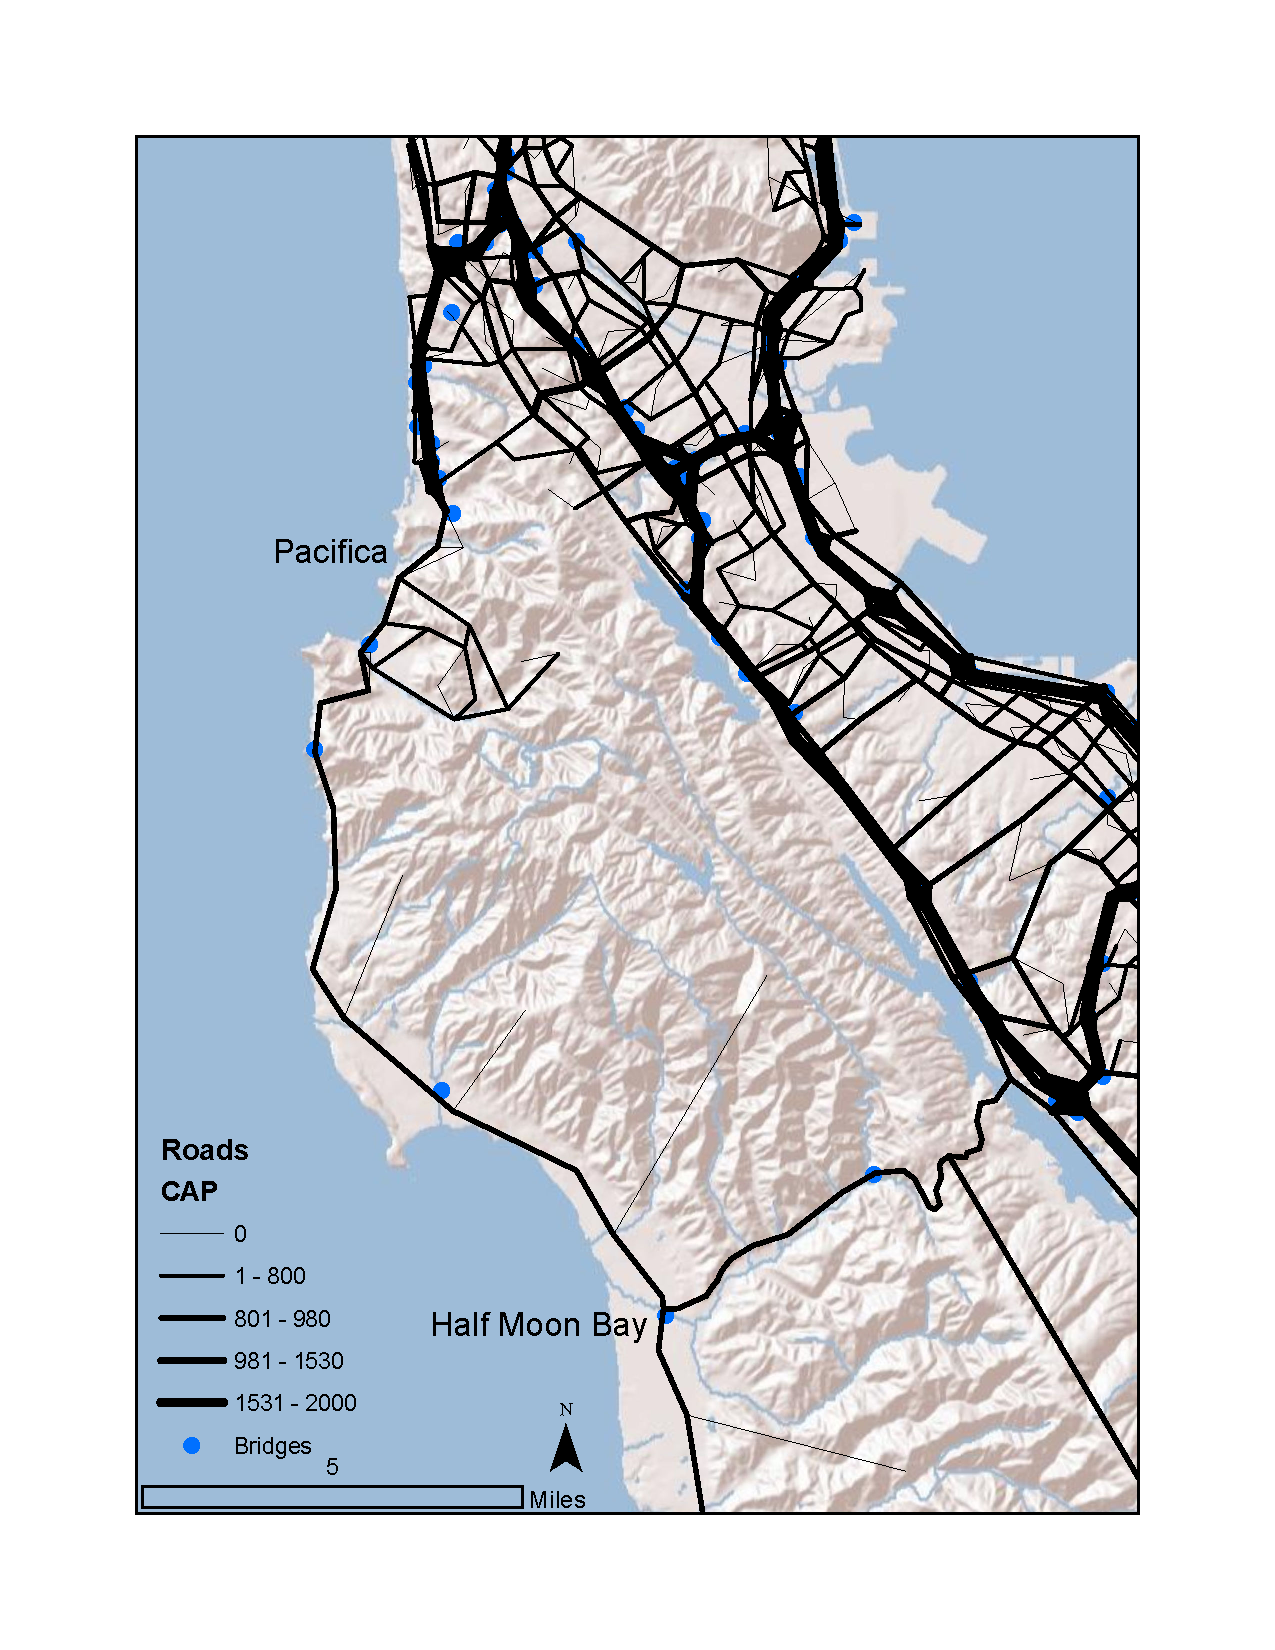
\includegraphics[height=7in]{FIGS/equity_hmb.pdf} 
%\caption{Differences in road access: limited roads in and out of Pacifica, CA, but an extra access highway for Half Moon Bay, CA.}
%\label{fig:pac}
%\end{figure*}

